\subsection{General Architecture}
\label{sec:CG-Architecture}

Our proposal relies on a middleware that embeds a \CEP engine for handling event processing, as depicted in Figure \ref{fig:Architecture}. Our tool offers a simulation mode, where devices are simulated as software components mimicking their actual execution, thus allowing to test \IOT scenarios without physical devices.

\begin{figure}%
	\centering  
	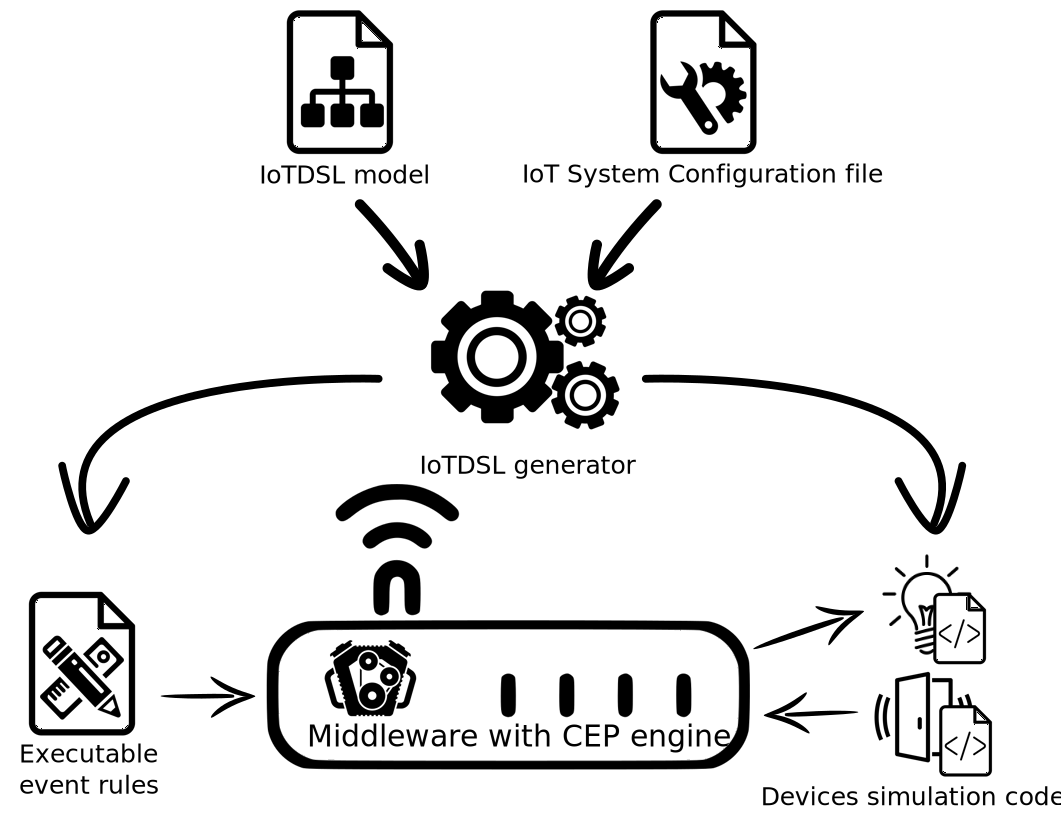
\includegraphics[width=.75\linewidth]{gen-archi.png}%
	\caption{General architecture of \IOTDSL framework}%
	\label{fig:Architecture}%
\end{figure}

The central element is the automatic code generator process: it produces executable code from \IOTDSL models and configuration files that define platform-specific details on the execution timing of devices (that the technicians set once and for all), and, for the purpose of our prototype, simulation code used to emulate the behaviour of the devices. The executable code is deployed into the \CEP engine running on a middleware, which reuses in simulation mode the code for communicating with the (abstract) devices. 

We are currently investigating how business rules could be broken down into smaller clusters that might be deployed directly into devices, assuming they offer sufficient battery and computation power. When addressing non-functional properties of devices, we envision the possibility of expressing technical specifications relative to the energy consumption and computation capabilities in a separate file that \IOTDSL would take into consideration to identify distributable rules.

